\documentclass{beamer}
\usepackage[utf8]{inputenc}

\usetheme{Madrid}
\usecolortheme{default}
\usepackage{amsmath,amssymb,amsfonts,amsthm}
\usepackage{txfonts}
\usepackage{tkz-euclide}
\usepackage{listings}
\usepackage{adjustbox}
\usepackage{array}
\usepackage{tabularx}
\usepackage{gvv}
\usepackage{lmodern}
\usepackage{circuitikz}
\usepackage{tikz}
\usepackage{graphicx}
\usepackage{mathtools}
\setbeamertemplate{page number in head/foot}[totalframenumber]

\usepackage{tcolorbox}
\tcbuselibrary{minted,breakable,xparse,skins}



\definecolor{bg}{gray}{0.95}
\DeclareTCBListing{mintedbox}{O{}m!O{}}{%
  breakable=true,
  listing engine=minted,
  listing only,
  minted language=#2,
  minted style=default,
  minted options={%
    linenos,
    gobble=0,
    breaklines=true,
    breakafter=,,
    fontsize=\small,
    numbersep=8pt,
    #1},
  boxsep=0pt,
  left skip=0pt,
  right skip=0pt,
  left=25pt,
  right=0pt,
  top=3pt,
  bottom=3pt,
  arc=5pt,
  leftrule=0pt,
  rightrule=0pt,
  bottomrule=2pt,
  toprule=2pt,
  colback=bg,
  colframe=orange!70,
  enhanced,
  overlay={%
    \begin{tcbclipinterior}
    \fill[orange!20!white] (frame.south west) rectangle ([xshift=20pt]frame.north west);
    \end{tcbclipinterior}},
  #3,
}
\lstset{
    language=C,
    basicstyle=\ttfamily\small,
    keywordstyle=\color{blue},
    stringstyle=\color{orange},
    commentstyle=\color{green!60!black},
    numbers=left,
    numberstyle=\tiny\color{gray},
    breaklines=true,
    showstringspaces=false,
}

\title 
{4.11.39}
\date{October 2, 2025}


\author 
{Vivek K Kumar - EE25BTECH11062}



\begin{document}


\frame{\titlepage}
\begin{frame}{Question}
Find the area of the region bounded by the lines $3x - 2y + 1 = 0$, $2x + 3y - 21 = 0$
and $x - 5y + 9 = 0$
\end{frame}

\begin{frame}{Variables used}
\begin{align}
\end{align}
\begin{table}[H]    
  \centering
  \begin{tabular}{|c|c|}
\hline
\textbf{Name} & \textbf{Value} \\ \hline
$\vec{A}$ & $\myvec{2 & 1 \\0 & 3}$ \\ \hline
\end{tabular}

  \caption{Variables used}
  \label{tab:4.11.39}
\end{table}

\end{frame}

\begin{frame}{Solution}
The given lines can be represented as 
\begin{align}
    \vec{n_1}^\top\vec{x} = c_1\\
    \vec{n_2}^\top\vec{x} = c_2\\
    \vec{n_3}^\top\vec{x} = c_3
\end{align}

Let the points of intersections of the given lines be represented as $\vec{A}, \vec{B}, \vec{C}$
\begin{align}
    \myvec{\vec{n_1} & \vec{n_2}}^\top\vec{A} = \myvec{c_1 \\ c_2}\\
    \myvec{\vec{n_2} & \vec{n_3}}^\top\vec{B} = \myvec{c_2 \\ c_3} \\
    \myvec{\vec{n_3} & \vec{n_1}}^\top\vec{C} = \myvec{c_3 \\ c_1} 
\end{align}
\end{frame}
\begin{frame}{Solution}
The area of the triangle can be then represented as
\begin{align}
    \frac{1}{2} \norm{\vec{A}-\vec{B}}\norm{\vec{C}-\vec{B}} \sqrt{1- \brak{\frac{\vec{n_2}^\top\vec{n_3}}{\norm{\vec{n_2}}\norm{\vec{n_3}}}} ^ 2}
\end{align}

Solving for $\vec{A}, \vec{B}, \vec{C}$
\begin{align}
    \myvec{3 & -2 \\ 2 & 3}\vec{A} = \myvec{-1 \\ 21} \\ 
   \implies \myaugvec{2}{3 & -2 & -1 \\ 2 & 3 & 21} \xleftrightarrow[]{R_2 \leftarrow R_2-2/3R_1} \myaugvec{2}{3 & -2 & -1 \\ 0 & 13/3 & 65/3}\\
   \vec{A} = \myvec{3 \\ 5}
\end{align}
\end{frame}

\begin{frame}{Solution}
\begin{align}
    \myvec{2 & 3 \\ 1 & -5}\vec{B} = \myvec{21 \\ -9} \\ 
    \implies \myaugvec{2}{2 & 3 & 21 \\ 1 & -5 & -9} \xleftrightarrow[]{R_2 \leftarrow R_2-1/2R_1} \myaugvec{2}{2 & 3 & 21 \\ 0 & -13/2 & -39/2}\\
   \vec{B} = \myvec{6 \\ 3}
\myvec{1 & -5 \\ 3 & -2}\vec{C} = \myvec{-9 \\ -1} \\ 
    \implies \myaugvec{2}{1 & -5 & -9 \\ 3 & -2 & -1} \xleftrightarrow[]{R_2 \leftarrow R_2-3R_1} \myaugvec{2}{1 & -5 & -9 \\ 0 & 13 & 26}\\
   \vec{C} = \myvec{1 \\ 2}
\end{align}
\end{frame}

\begin{frame}{Solution}
Area of the triangle from the previous equations is
\begin{align}
    \frac{1}{2}\norm{\myvec{-3 & 2}^\top}\norm{\myvec{-5 & -1}^\top}\sqrt{1 - \brak{\frac{-13}{13\sqrt{2}}}^2} = \frac{13}{2}
\end{align}
\end{frame}

\begin{frame}[fragile]
    \frametitle{Python - Importing libraries and checking system}
    \begin{lstlisting}
import sys
import numpy as np
import numpy.linalg as LA
import matplotlib.pyplot as plt
import matplotlib.image as mpimg
import math

from libs.line.funcs import *
from libs.triangle.funcs import *
from libs.conics.funcs import circ_gen

import subprocess
import shlex

print('Using termux?(y/n)')
y = input()
\end{lstlisting}
\end{frame}

\begin{frame}[fragile]
    \frametitle{Python - Writing required points and direction vectors}
    \begin{lstlisting}
m1 = np.array([2, 3]).reshape(-1,1)
m2 = np.array([-3, 2]).reshape(-1,1)
m3 = np.array([5, 1]).reshape(-1,1)
A = np.array([3, 5]).reshape(-1,1)
B = np.array([6, 3]).reshape(-1,1)
C = np.array([1, 2]).reshape(-1,1)
\end{lstlisting}
\end{frame}

\begin{frame}[fragile]
    \frametitle{Python - Generating points and plotting}
    \begin{lstlisting}
p_l1 = line_gen(A-1.5*m1, A+1.5*m1)
p_l2 = line_gen(B-1.5*m2, B+1.5*m2)
p_l3 = line_gen(C-1.5*m3, C+1.5*m3)

fig = plt.figure()
ax = fig.add_subplot(111)

ax.plot(p_l1[0, :], p_l1[1, :], label = '3x-2y+1=0')
ax.plot(p_l2[0, :], p_l2[1, :], label = '2x+3y-21=0')
ax.plot(p_l3[0, :], p_l3[1, :], label = 'x-5y+9=0')
\end{lstlisting}
\end{frame}

\begin{frame}[fragile]
    \frametitle{Python - Labelling points}
    \begin{lstlisting}
pts = np.block([A, B, C])
labels = ['A(3,5)', 'B(6,3)', 'C(1,2)']
ax.scatter(pts[0, :], pts[1, :])
for i, txt in enumerate(labels):
        ax.text(pts[0, i], pts[1, i], s=txt)

ax.set_xlabel('$X$')
ax.set_ylabel('$Y$')
ax.legend(loc='best')
ax.grid(True) 
ax.axis('equal')
    \end{lstlisting}
\end{frame}

\begin{frame}[fragile]
    \frametitle{Python - Saving figure and opening it}
    \begin{lstlisting}
fig.savefig('../figs/fig.png')
print('Saved figure to ../figs/fig.png')

if(y == 'y'):
    subprocess.run(shlex.split('termux-open ../figs/fig.png'))
else:
    subprocess.run(["open",  "../figs/fig.png"])
    \end{lstlisting}
\end{frame}


\begin{frame}{Plot-Using only Python}
    \centering
    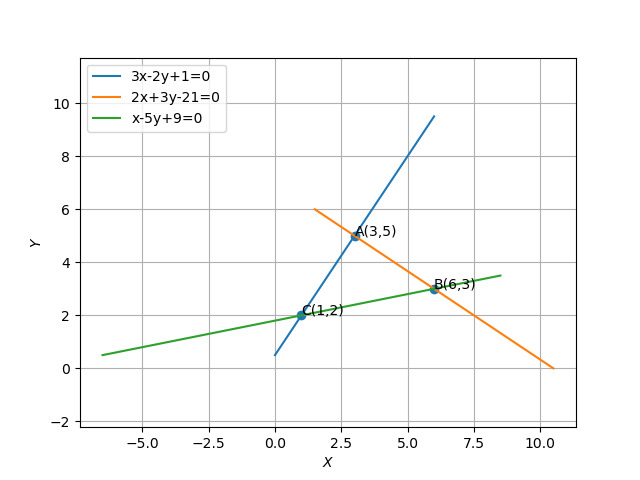
\includegraphics[width=\columnwidth, height=0.8\textheight, keepaspectratio]{../figs/fig.png}     
\end{frame}

\begin{frame}[fragile]
    \frametitle{C Code (0) - Importing libraries}

    \begin{lstlisting}
#include <stdio.h>
#include <stdlib.h>
#include <string.h>
#include <math.h>
#include <sys/socket.h>
#include <netinet/in.h>
#include <unistd.h>
#include "libs/matfun.h"
#include "libs/geofun.h"
    \end{lstlisting}
\end{frame}
\begin{frame}[fragile]
    \frametitle{C Code (1) - Function to Generate Points on a Line}

    \begin{lstlisting}

void point_gen(FILE *p_file, double **A, double **B, int rows, int cols, int npts){
    for(int i = 0; i <= npts; i++){
     double **output = Matadd(A, Matscale(Matsub(B, A, rows, cols), rows, cols, (double)i/npts), rows, cols);
     fprintf(p_file, "%lf, %lf\n", output[0][0], output[1][0]);
     freeMat(output, rows);
    }
}

    \end{lstlisting}
\end{frame}


\begin{frame}[fragile]
    \frametitle{C Code (2) - Function to write points b/w given points to a file}

    \begin{lstlisting}
void write_points(double x1, double y1, double x2, double y2, double x3, double y3, int npts){
    int m = 2;
    int n = 1;

    double **A = createMat(m, n);
    double **B = createMat(m, n);
    double **C = createMat(m, n);

    B[0][0] = x2;
    B[1][0] = y2;
    \end{lstlisting}
\end{frame}
\begin{frame}[fragile]
    \frametitle{C Code (2) - Function to write points b/w given 2 points to a file}

    \begin{lstlisting}
    A[0][0] = x1;
    A[1][0] = y1;
    C[0][0] = x3;
    C[1][0] = y3;
    double **L1_1 = Matsub(A, Matscale(Matsub(B, A, m, n), m, n, -1.5), m, n);
    double **L1_2 = Matsub(A, Matscale(Matsub(B, A, m, n), m, n, 1.5), m, n);
    double **L2_1 = Matsub(B, Matscale(Matsub(C, B, m, n), m, n, -1.5), m, n);
    double **L2_2 = Matsub(B, Matscale(Matsub(C, B, m, n), m, n, 1.5), m, n);
    double **L3_1 = Matsub(C, Matscale(Matsub(C, A, m, n), m, n, -1.5), m, n);
    double **L3_2 = Matsub(C, Matscale(Matsub(C, A, m, n), m, n, 1.5), m, n);
    \end{lstlisting}
\end{frame}

\begin{frame}[fragile]
    \frametitle{C Code (2) - Function to write points b/w given 2 points to a file}
    \begin{lstlisting}
    FILE *p_file;
    p_file = fopen("plot.dat", "w");
    
    if(p_file == NULL)
        printf("Error opening one of the data files\n");
    point_gen(p_file, L1_1, L1_2, m, n, npts);
    point_gen(p_file, L2_1, L2_2, m, n, npts);
    point_gen(p_file, L3_1, L3_2, m, n, npts);
    \end{lstlisting}
\end{frame}

\begin{frame}[fragile]
    \frametitle{C Code (2) - Function to write points b/w 2 points to a file}
    \begin{lstlisting}
    freeMat(A, m);
    freeMat(B, m);
    freeMat(C, m);
    freeMat(L1_1, m);
    freeMat(L1_2, m);
    freeMat(L2_1, m);
    freeMat(L2_2, m);
    freeMat(L3_1, m);
    freeMat(L3_2, m);

    fclose(p_file);
}
    \end{lstlisting}
\end{frame}

\begin{frame}[fragile]
    \frametitle{Python Code (0) - Importing libraries and checking system}
    \begin{lstlisting}
import numpy as np
import matplotlib.pyplot as plt
import ctypes
import os
import sys
import subprocess
import math

print('Using termux? (y/n)')
termux = input()
\end{lstlisting}
\end{frame}

\begin{frame}[fragile]
    \frametitle{Python Code (1) - Using Shared Object}
    \begin{lstlisting}
lib_path = os.path.join(os.path.dirname(__file__), 'plot.so')
my_lib = ctypes.CDLL(lib_path)

my_lib.write_points.argtypes = [ctypes.c_double, ctypes.c_double, ctypes.c_double, ctypes.c_double, ctypes.c_double, ctypes.c_double, ctypes.c_int]
my_lib.write_points.restype = None
A = np.array([3, 5]).reshape(-1, 1)
B = np.array([6, 3]).reshape(-1, 1)
C = np.array([1, 2]).reshape(-1, 1)
npts = 20000
\end{lstlisting}
\end{frame}

\begin{frame}[fragile]
    \frametitle{Python Code (2) - Loading points and plotting them}
    \begin{lstlisting}
fig = plt.figure()
ax = fig.add_subplot(111)
labels = ['3x-2y+1=0', '2x+3y-21=0', 'x-5y+9=0']
point_labels = ['A(3, 5)', 'B(6, 3)', 'C(1,2)']
pts = np.block([A, B, C])

for i,label in enumerate(labels):
    points = np.loadtxt('plot.dat', delimiter = ',', usecols=(0,1))[i*(npts+1):(i+1)*(npts+1)]
    ax.plot(points[:, 0], points[:, 1], label = label)
    ax.text(pts[0, i], pts[1, i], s=point_labels[i])
\end{lstlisting}
\end{frame}

\begin{frame}[fragile]
    \frametitle{Python Code (3) - Labelling plot}
    \begin{lstlisting}
        ax.set_xlabel('$X$')
        ax.set_ylabel('$Y$')
        ax.legend(loc='best')
        ax.grid() 
        ax.axis('equal')
    \end{lstlisting}
\end{frame}

\begin{frame}[fragile]
    \frametitle{Python Code (4) - Saving and displaying plot}
    \begin{lstlisting}
fig.savefig('../figs/fig2.png')
print('Saved figure to ../figs/fig2.png')

if(termux == 'y'):
    subprocess.run(shlex.split('termux-open ../figs/fig2.png'))
else:
    subprocess.run(["open",  "../figs/fig2.png"])
\end{lstlisting}
\end{frame}

\begin{frame}{Plot-Using Both C and Python}
    \centering
    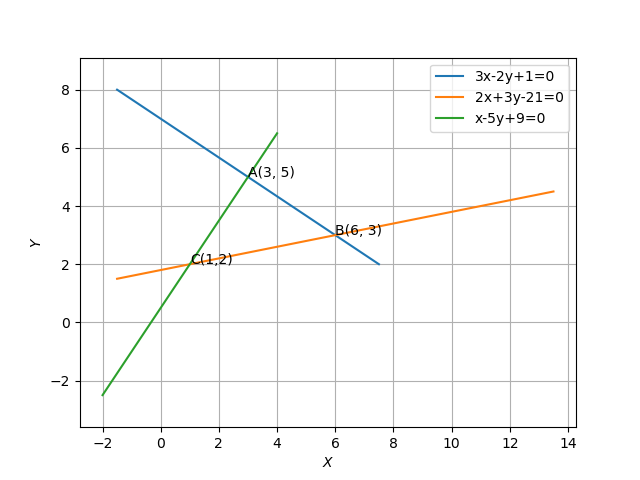
\includegraphics[width=\columnwidth, height=0.8\textheight, keepaspectratio]{../figs/fig2.png}     
\end{frame}

\end{document}